\documentclass[10pt]{IEEEtran}
\usepackage[spanish]{babel}
\usepackage[utf8]{inputenc}
\usepackage{graphicx}
\usepackage{subfigure} 
\usepackage{amsmath}
\usepackage{float}



\title {Operación XOR de manera cruzada en mapas Renyi donde $i \neq j$, aplicación de pruebas NIST.}

\author{\IEEEauthorblockN{Marcos Daniel Calderón Calderón}\\
\IEEEauthorblockA{Maestría en Ciencias de la Computación\\
Centro de Investigación en Matemáticas (CIMAT)\\
Guanajuato , Gto.\\
marcos.calderon@cimat.mx}}


\begin{document}
\maketitle
\begin{abstract}
En este reporte se explica de manera detallada el funcionamiento de una operación XOR de manera cruzada entre la parte inferior y superior de dos números por mapas caóticos Renyi. Pero ahora se tiene la restricción de que el valor de $i$ sea diferente del valor de $j$.
\end{abstract}
\section{Introducción.}

EL mapa caótico Renyi tiene la siguiente forma:

\begin{equation}
f(k)=  \left(  q2^{n-i}k +  \lfloor \frac{k}{2^{j}} \rfloor   \right) \mod{ 2^{n}}
\end{equation}.




El esquema que se para su combinación es el siguiente:
\begin{figure}[H]
\centering
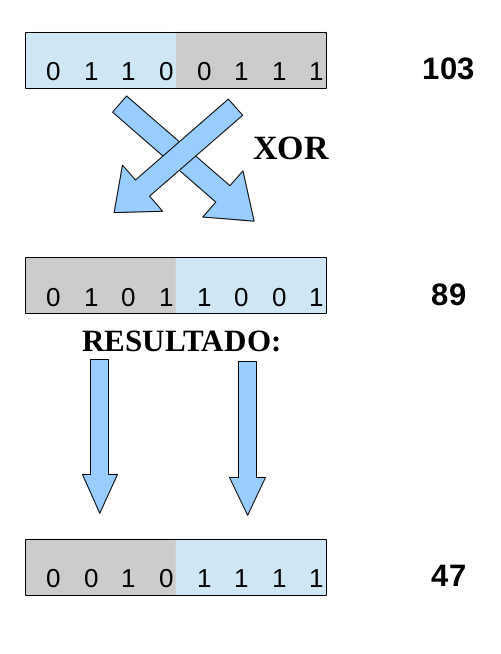
\includegraphics[width=7cm]{es.jpg}
\caption{Esquema de intercambio.}
\label{vovo}
\end{figure}


Ahora, para los ejemplos que se muestran aquí se utilizan 32 bits, esto significa que se van a dividir los datos generados por los mapas caóticos en dos partes: cada una de 16 bits. También, en este caso, necesitamos un nuevo valor para a: $(a = 2^{16}-1= 65,535)$



\section{Ejemplo 1.}

\subsection{Procedimiento.}
Para este ejemplo, se han elegido los siguientes valores:

\begin{itemize}
\item Mapa 1: $i  = 5 \quad j = 7$.


\item Mapa 2: $i = 6 \quad j = 14$.
\end{itemize}

Ahora, es necesario elegir un valor de $q$ adecuado, en este ejemplo, utilizamos los siguientes:

\begin{itemize}
\item Mapa 1: $q = 13.$
\item Mapa 2: $q = 19.$
\end{itemize}


Ahora, es necesario calcular el parámetro que se forma de la expresión:  
\begin{equation}
\beta = q 2^{n-i}
\end{equation}
con base en lo anterior, se encontraron los siguientes parámetros para el mapa 1 y el mapa 2 respectivamente:

\begin{itemize}
\item $\beta_{1}=1744830464$.
\item $\beta_{2}=1275068416$.
\end{itemize}


 
También es importante elegir el tipo de dato que se va a utilizar para almacenar los valores generados por los mapas, en este caso se eligió el tipo de dato \textbf{unsigned long} (se utilizó un equipo con arquitectura de 32 bits, donde este tipo de dato tiene un tamaño de 32 bits).

Se generaron 80,000 valores  a la hora de relacionar los valores de los dos mapas con la operación XOR. Como cada valor está formado de 32 bits, se  obtiene un total de $2,560,000$ bits para la aplicación de pruebas NIST.



Se utilizó el siguiente código para la ejecución de las pruebas NIST:


\begin{itemize}
\item \textbf{./assess 2560000}
\item User Prescribed Input File: \textbf{dosRenyisIntercambio1idifj.dat}
\item    Enter 0 if you DO NOT want to apply all of the
         statistical tests to each sequence and 1 if you DO. Enter chice: \textbf{1}
                  
\item  How many bitstreams? \textbf{1}

\item Input File Format:
    [0] ASCII - A sequence of ASCII 0's and 1's
    [1] Binary - Each byte in data file contains 8 bits of data

   Select input mode:  \textbf{1}
\end{itemize}

\subsection{Resultados.}
Los resultados no son buenos, de hecho ninguna prueba es aprobada.


 
\section{Ejemplo 2.}

\subsection{Procedimiento.}
Para el ejemplo 2, se eligieron los siguientes parámetros:

\begin{itemize}
\item Mapa 1: $i = 8 \quad j = 13$.
\item Mapa 2: $i = 10, j = 15$.
\end{itemize}

Ahora, es necesario elegir un valor de $q$ adecuado, en este ejemplo, utilizamos los siguientes:

\begin{itemize}
\item Mapa 1: $q = 29$.
\item Mapa 2: $q = 31$.
\end{itemize}


Ahora, es necesario calcular el parámetro que se forma de la expresión:  
\begin{equation}
\beta = q 2^{n-i}
\end{equation}
con base en lo anterior, se encontraron los siguientes parámetros para el mapa 1 y el mapa 2 respectivamente:

\begin{itemize}
\item $\beta_{1}=$.
\item $\beta_{2}=$.
\end{itemize}




Se utilizó el siguiente código para la ejecución de las pruebas NIST:


\begin{itemize}
\item \textbf{./assess 2560000}
\item User Prescribed Input File: \textbf{dosRenyisIntercambio2idifj.dat}
\item    Enter 0 if you DO NOT want to apply all of the
         statistical tests to each sequence and 1 if you DO. Enter chice: \textbf{1}
                  
\item  How many bitstreams? \textbf{1}

\item Input File Format:
    [0] ASCII - A sequence of ASCII 0's and 1's
    [1] Binary - Each byte in data file contains 8 bits of data

   Select input mode:  \textbf{1}
\end{itemize}





\subsection{Resultados.}

No se obtuvieron buenos resultados: no se aprobó ninguna prueba NIST.


 

\section{Conclusiones.}



\onecolumn
\section{Anexos.}




\end{document}


